\chapter{Struktur af rapporten}\label{chap:struktur-af-problemanalyse}

I dette afsnit, beskrives strukturen af rapporten.
Strukturen er baseret på beskrivelsen af et informationssystem fra \citet{Laudon1999}.
Komponenterne i et informationssystem er illustreret i \myref{fig:kontekstmodel}.

\begin{figure}[htbp]
  \centering
  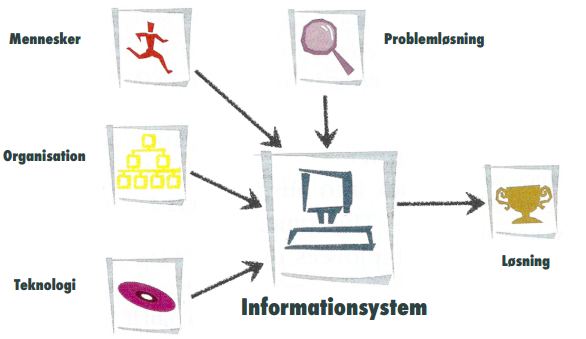
\includegraphics{images/kontekstmodel/metode.png}
  \caption[Metode for Kontekstmodellen]{Illustration af elementerne i et informationssystem. Kilde:
  \protect\citet{Laudon1999}}
  \label{fig:kontekstmodel}
\end{figure}


\section{Informationssystem}\label{sec:Informationssystem}

Et informationssystem bruges til at effektivisere en arbejdsproces og hjælper med at holde fokus, så arbejdet bliver udført tilfredsstillende. 
For at udvikle et godt informationssystem, skal man indsamle viden om mennesker, organisation og teknologi. 
Når informationssystemet er udviklet, består det af tre processer: Indsamling af data, behandling af dataene og formidling af dataene. 
De tre elementer bruges til at undersøge, hvad der skal tages hensyn til under problemløsningsdelen, og vil blive beskrevet herefter.

\subsection{Mennesker}\label{subsec:mennesker}

Elementet \textit{mennesker} omhandler de personer, som har en interesse i, at en given problemstilling løses. 
Det kan være brugeren af det program, der bliver lavet, samt andre, som får gavn af en løsning.
Man undersøger bl.a. brugerens evner, da programmet skal laves på en sådan måde, at brugeren har den fornødne kunnen, til at betjene programmet.
Brugerens behov undersøges også, så man får alle de funktioner med, som er nødvendige for et brugbart program.


\subsubsection{Organisation}\label{subsec:organisation}

Elementet \textit{organisation} undersøges hvor og hvordan problemerne opstår, derudover undersøges hvilke regler og værdier organisationen har, for at kunne tage højde for disse under problemløsningen.


\subsection{Teknologi}\label{subsec:Teknologi}

Elementet \textit{teknologi} omhandler de teknologier, som anvendes til at løse en informationssystemrelevant problemstilling.
Derfor vil der blive undersøgt andre informationssystemer, der er rettet imod samme gruppe, som dette projekt.


\subsection{Problemløsning}
Ud fra de tre førnævnte elementer er der blevet indsamlet data, hvilket skal tages i betragtning i forhold til et informationssystem.
Disse anvendes til at opstille krav, som problemløsningen skal tage hensyn til.
Kravene vil blive brugt under resten af problemløsningen.


\section{Rapportens opbygning}\label{sec:rapportens-opbygning}

Først bliver menneskedelen behandlet, i form af en interessentanalyse, hvorefter vil organisationselementet blive berørt.
Derefter bliver der skrevet om teknologier, hvorefter de tre elementer munder ud i en problemafgrænsning og en problemformulering.
Informationen, indsamlet igennem problemanalysen såvel som problemformuleringen, benyttes til at opstille krav for problemløsningen, efterfulgt af en beskrivelse af informationssystemet. 
Rapporten afrundes med en diskussion af rapporten, samt en opsamling på informationssystemet i form af en konklusion. Desuden ses der på en eventuel videreudvikling og tilføjelser til informationssystemet såvel som andre potentielle anvendelser.